The central dogma of molecular biology (Fig. \ref{fig:central_dogma}) describes the flow of information from DNA (deoxyribonucleic acid), 
through RNA (ribonucleic acid) into proteins. 
During the transcription process,
DNA is duplicated into a complementary RNA strand, 
which acts as messenger to deliver the information to the ribosome. 
Ribosomes use the code embedded in the messenger RNA (mRNA) to construct 
a protein in a process called translation (\cite{crick1970}).

DNA is a linear polymer with a fixed backbone from which can extend 4 different bases: 
adenine (A),
cytosine (C), 
guanine (G),
and thymine (T). 
These bases combine into specific Watson-Crick base pairs,
held together by hydrogen bonds. 
This way, two single strands of DNA can combine into a double helix.
Each strand contains all information to form the other, 
providing a template for the DNA replication mechanism. 
These features combined with its robust nature make DNA the ideal candidate for storage
and heredity of information (\cite{berg2015}).

During transcription, 
the same Watson-Crick base pairing rules are used to copy the information to mRNA. 
The only difference being that the base thymine is replaced by an uracil base. 
The protein RNA polymerase synthesises a complementary strand of mRNA by reading the sense thread of dsDNA. 
The mRNA is transported through the cytoplasm to the ribosomes, 
which can be seen as the protein factories of the cell. 
Ribosomes read the mRNA template three bases at a time, also known as codons. 
Each codon is translated into a specific amino acid.
There are 64 different codons, yet only 20 distinct amino acids. 
This means that multiple codons encode the same amino acid. 
Codon for codon, the mRNA is translated into a linear polymer of amino acids.

~\begin{figure}[h!]
	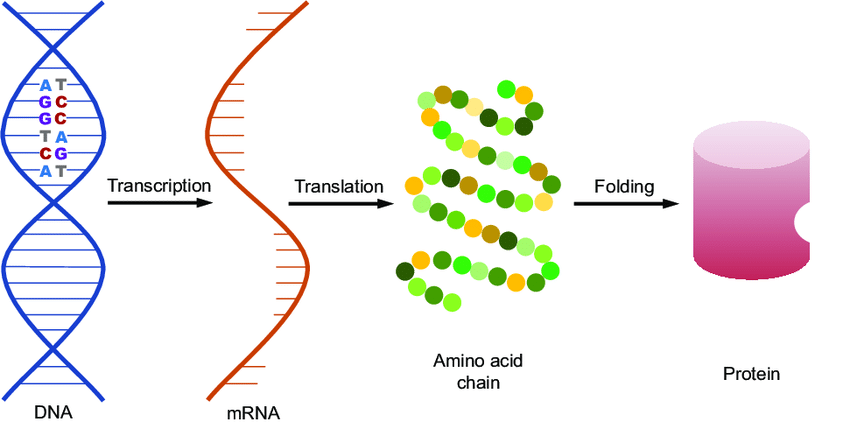
\includegraphics[width=\linewidth]{./literature_review/central_dogma/img/central_dogma.png}
	\caption{
	\textbf{Central dogma of molecular biology.}
	It describes the flow of molecular information, 
	starting from DNA, 
	through RNA, 
	and ending as a amino acid sequence. 
	Subsequently, this sequence folds into a functional protein.
	The transition from DNA to RNA is called transcription, 
	the transition from RNA to a protein is called translation
	(from \cite{cichonska2018}).	
	}
	\label{fig:central_dogma}
~\end{figure}
